\documentclass[a4paper,12pt]{article}
\usepackage[utf8]{inputenc}
\usepackage[T1]{fontenc}
\usepackage{lmodern}
\usepackage[english]{babel}
\usepackage{amsmath, amssymb, amsthm, physics}
\usepackage{graphicx}
\usepackage{xcolor}
\usepackage{tikz}
\usepackage{pgfplots}
\pgfplotsset{compat=1.18}
\usepackage{setspace}
\usepackage{tcolorbox}
\usepackage{booktabs}
\usepackage{siunitx}
\usepackage{textalpha}
\usepackage{textgreek}

\usepackage{hyperref}
\hypersetup{
	colorlinks=true,
	linkcolor=blue,
	filecolor=blue,
	citecolor=blue,
	urlcolor=blue,
	bookmarks=true,
	bookmarksopen=true,
	pdftitle={Dark Energy in the T0 Model: A Mathematical Analysis of Energy Dynamics},
	pdfauthor={Johann Pascher},
}

\usepackage{cleveref}

\newtheorem{theorem}{Theorem}[section]
\newtheorem{lemma}[theorem]{Lemma}
\newtheorem{proposition}[theorem]{Proposition}
\newtheorem{corollary}[theorem]{Corollary}

\theoremstyle{definition}
\newtheorem{definition}[theorem]{Definition}
\newtheorem{example}[theorem]{Example}

\theoremstyle{remark}
\newtheorem{remark}[theorem]{Remark}
\renewcommand{\proofname}{Proof}

\newcommand{\Tfield}{T(x)}

\begin{document}
	
	\title{Dark Energy in the T0 Model: \\A Mathematical Analysis of Energy Dynamics}
	\author{Johann Pascher}
	\date{March 26, 2025}
	\maketitle
	
	\begin{abstract}
		This work develops a detailed mathematical analysis of dark energy within the framework of the T0 model with absolute time and variable mass. Unlike the $\Lambda$CDM standard model, dark energy is not considered a driving force of cosmic expansion but a dynamic medium for energy exchange in a static universe. The document derives the corresponding field equations, characterizes energy transfer rates, analyzes the radial density profile of dark energy, and explains the observed redshift as a result of photon energy loss. Finally, specific experimental tests are proposed to distinguish between this interpretation and the standard model.
	\end{abstract}
	
	\tableofcontents
	\newpage
	
	\section{Introduction}
	The discovery of accelerated cosmic expansion through supernova observations in the late 1990s led to the introduction of dark energy as the dominant component of the universe. In the standard cosmological model ($\Lambda$CDM), dark energy is modeled as a cosmological constant ($\Lambda$) with negative pressure, accounting for approximately 68\% of the universe’s energy content and driving the accelerated expansion.
	
	This work pursues an alternative approach based on the T0 model, where time is absolute and particle mass varies. Within this framework, dark energy is not a driving force of expansion but a medium for energy exchange interacting with matter and radiation. Cosmic redshift arises not from spatial expansion but from photon energy loss to dark energy.
	
	In the following, we will mathematically refine this approach, derive the necessary field equations, determine the energy density and distribution of dark energy, and analyze the consequences for astronomical observations. We will then explore experimental tests that could differentiate between the T0 model and the standard model.
	
	\section{Fundamentals of the T0 Model for Dark Energy}
	We first summarize the foundational concepts of the T0 model concerning dark energy.
	
	\subsection{Fundamental Assumptions}
	Unlike the standard model, where spacetime is dynamic and expands while rest mass remains constant, the T0 model postulates:
	
	\begin{tcolorbox}[colback=blue!5!white,colframe=blue!75!black,title=Fundamental Assumptions of the T0 Model]
		\begin{align}
			&\text{1. Time $T_0$ is absolute and universally constant.} \\
			&\text{2. Mass varies as $m = \gamma m_0$, where $\gamma = \frac{1}{\sqrt{1-v^2/c_0^2}}$.} \\
			&\text{3. The total energy of the universe is constant.} \\
			&\text{4. Redshift results from energy loss: $E_2 = E_1(1+z)^{-1}$.}
		\end{align}
	\end{tcolorbox}
	
	For dark energy, this implies it is not a uniform background density expanding space but a dynamic field capable of exchanging energy with matter and radiation, while the universe’s total energy remains constant.
	
	\subsection{Dark Energy as a Dynamic Field}
	Dark energy in the T0 model is modeled as a scalar field $\phi_{DE}$ interacting with matter and radiation. Its energy density is not constant but exhibits a spatial structure:
	
	\begin{equation}
		\rho_{DE}(r) = \frac{\kappa}{r^2}
	\end{equation}
	
	where $\kappa$ is a constant and $r$ denotes radial distance. This $1/r^2$ profile starkly contrasts with the constant energy density $\rho_\Lambda$ of the cosmological constant in the standard model.
	
	The coupling between dark energy and matter/radiation can be described by an interaction term in the Lagrangian density:
	
	\begin{equation}
		\mathcal{L}_{int} = -\frac{\beta}{M_{Pl}} \phi_{DE} T^{\mu}_{\mu}
	\end{equation}
	
	Here, $\beta$ is a dimensionless coupling constant, $M_{Pl}$ is the Planck mass, and $T^{\mu}_{\mu}$ is the trace of the energy-momentum tensor of matter and radiation.
	
	\section{Field-Theoretic Description of Dark Energy}
	We now develop a complete field-theoretic description of dark energy in the T0 model.
	
	\subsection{Lagrangian Density of Dark Energy}
	The complete Lagrangian density for the dark energy field is:
	
	\begin{equation}
		\mathcal{L}_{DE} = -\frac{1}{2}\partial_\mu \phi_{DE} \partial^\mu \phi_{DE} - V(\phi_{DE}) - \frac{\beta}{M_{Pl}} \phi_{DE} T^{\mu}_{\mu} - \frac{1}{2}\xi \phi_{DE}^2 R
	\end{equation}
	
	where:
	\begin{itemize}
		\item $\partial_\mu \phi_{DE} \partial^\mu \phi_{DE}$ is the kinetic term,
		\item $V(\phi_{DE})$ is the self-interaction potential,
		\item $\frac{\beta}{M_{Pl}} \phi_{DE} T^{\mu}_{\mu}$ is the coupling to matter and radiation,
		\item $\frac{1}{2}\xi \phi_{DE}^2 R$ is a non-minimal coupling to spacetime curvature $R$.
	\end{itemize}
	
	For a static universe in the T0 model, we must choose a suitable potential $V(\phi_{DE})$ that allows a stable equilibrium:
	
	\begin{equation}
		V(\phi_{DE}) = \frac{1}{2}m_{\phi}^2\phi_{DE}^2 + \lambda \phi_{DE}^4
	\end{equation}
	
	where $m_{\phi}$ is the mass of the dark energy field and $\lambda$ is the self-coupling constant.
	
	\subsection{Field Equations of Dark Energy}
	From the Lagrangian density, the Euler-Lagrange equations for the dark energy field are:
	
	\begin{equation}
		\Box\phi_{DE} - \frac{dV}{d\phi_{DE}} - \frac{\beta}{M_{Pl}}T^{\mu}_{\mu} - \xi \phi_{DE} R = 0
	\end{equation}
	
	which simplifies to:
	
	\begin{equation}
		\Box\phi_{DE} - m_{\phi}^2\phi_{DE} - 4\lambda\phi_{DE}^3 - \frac{\beta}{M_{Pl}}T^{\mu}_{\mu} - \xi \phi_{DE} R = 0
	\end{equation}
	
	For a static, spherically symmetric system, this reduces to:
	
	\begin{equation}
		\frac{1}{r^2}\frac{d}{dr}\left(r^2\frac{d\phi_{DE}}{dr}\right) = m_{\phi}^2\phi_{DE} + 4\lambda\phi_{DE}^3 + \frac{\beta}{M_{Pl}}T^{\mu}_{\mu} + \xi \phi_{DE} R
	\end{equation}
	
	\subsection{Energy Density Profile of Dark Energy}
	For a massless field ($m_{\phi} \approx 0$) and negligible curvature ($\xi R \approx 0$), the field equation simplifies to:
	
	\begin{equation}
		\frac{1}{r^2}\frac{d}{dr}\left(r^2\frac{d\phi_{DE}}{dr}\right) = 4\lambda\phi_{DE}^3 + \frac{\beta}{M_{Pl}}T^{\mu}_{\mu}
	\end{equation}
	
	We seek a solution reproducing the observed $1/r^2$ density profile of dark energy. For large distances $r$, where $T^{\mu}_{\mu} \approx 0$ (negligible matter density), the self-interaction term $\lambda$ dominates. Using an ansatz $\phi_{DE}(r) \propto r^{-\alpha}$, substitution and coefficient comparison yield $\alpha = 1/2$, so:
	
	\begin{equation}
		\phi_{DE}(r) \approx \left(\frac{1}{8\lambda}\right)^{1/3} r^{-1/2} \quad \text{for } r \gg r_0
	\end{equation}
	
	The energy density of dark energy is then:
	
	\begin{equation}
		\rho_{DE}(r) \approx \frac{1}{2}\left(\frac{d\phi_{DE}}{dr}\right)^2 + \frac{1}{2}m_{\phi}^2\phi_{DE}^2 + \lambda\phi_{DE}^4 \approx \frac{\kappa}{r^2}
	\end{equation}
	
	with $\kappa \propto \lambda^{-2/3}$. This $1/r^2$ profile matches the requirements for explaining flat galaxy rotation curves.
	
	\begin{figure}[h]
		\centering
		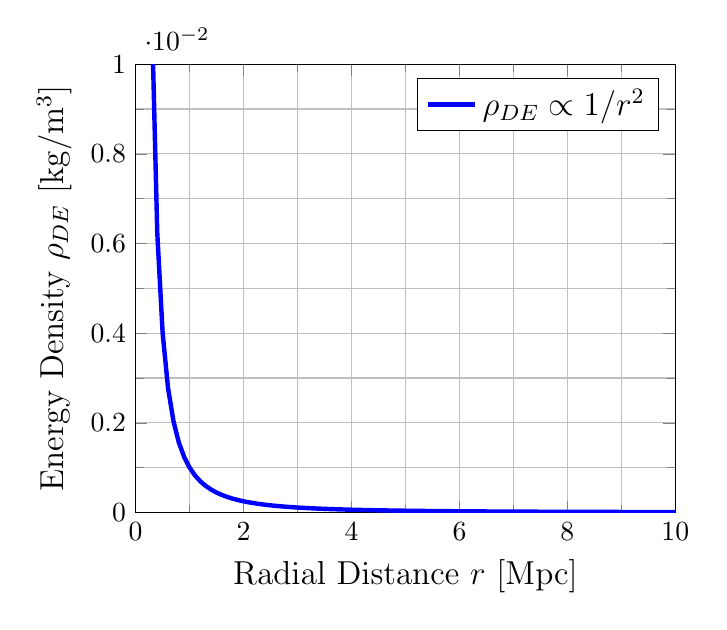
\begin{tikzpicture}
			\begin{axis}[
				xlabel={Radial Distance \(r\) [Mpc]},
				ylabel={Energy Density \(\rho_{DE}\) [kg/m\(^3\)]},
				xlabel style={font=\large},
				ylabel style={font=\large},
				tick label style={font=\normalsize},
				xmin=0, xmax=10,
				ymin=0, ymax=0.01,
				legend pos=north east,
				legend style={font=\large},
				grid=both,
				minor tick num=1
				]
				\addplot[blue, ultra thick, domain=0.1:10, samples=100] {0.001/(x^2)};
				\legend{\(\rho_{DE} \propto 1/r^2\)}
			\end{axis}
		\end{tikzpicture}
		\caption{Energy density profile of dark energy in the T0 model as a function of radial distance.}
	\end{figure}
	
	\section{Energy Exchange and Redshift}
	A key aspect of the T0 model is interpreting cosmic redshift as a result of photon energy loss to dark energy, not spatial expansion.
	
	\subsection{Photon Energy Loss}
	Consider a photon moving through the dark energy field. The photon’s energy change is described by:
	
	\begin{equation}
		\frac{dE_{\gamma}}{dx} = -\alpha E_{\gamma}
	\end{equation}
	
	where $\alpha$ is the absorption rate. This equation has the solution:
	
	\begin{equation}
		E_{\gamma}(x) = E_{\gamma,0} e^{-\alpha x}
	\end{equation}
	
	where $E_{\gamma,0}$ is the initial photon energy and $x$ is the distance traveled.
	
	The redshift $z$ is defined as:
	
	\begin{equation}
		1 + z = \frac{E_0}{E} = \frac{\lambda_{obs}}{\lambda_{emit}} = e^{\alpha d}
	\end{equation}
	
	where $d$ is the distance. For small $z$ (local distances):
	
	\begin{equation}
		z \approx \alpha d
	\end{equation}
	
	To ensure consistency with the observed Hubble relation $z \approx H_0 d/c$:
	
	\begin{equation}
		\alpha = \frac{H_0}{c} \approx 2.3 \times 10^{-28} \text{ m}^{-1}
	\end{equation}
	
	where $H_0 \approx 70 \text{ km/s/Mpc}$ is the Hubble constant.
	
	The energy transfer to the dark energy field can be further refined using the intrinsic time concept $\Tfield = \frac{\hbar}{mc^2}$. For photons, intrinsic time is defined as $\Tfield = \frac{\hbar}{E_{\gamma}} e^{\alpha x}$, with $\alpha = \frac{H_0}{c}$ as the absorption rate.
	
	\subsection{Energy Transfer to Dark Energy}
	The energy lost by the photon is transferred to the dark energy field. Energy conservation requires:
	
	\begin{equation}
		\frac{d}{dt}(E_{\gamma} + E_{DE}) = 0
	\end{equation}
	
	The rate at which dark energy gains energy is:
	
	\begin{equation}
		\frac{dE_{DE}}{dt} = -\frac{dE_{\gamma}}{dt} = \alpha c E_{\gamma}
	\end{equation}
	
	For the dark energy density, this implies:
	
	\begin{equation}
		\frac{d\rho_{DE}}{dt} = \alpha c \rho_{\gamma}
	\end{equation}
	
	where $\rho_{\gamma}$ is the photon energy density.
	
	\subsection{Energy Balance Equation}
	In a static universe with constant total energy, we must consider the energy balance. The total energy density $\rho$ comprises:
	
	\begin{equation}
		\rho_{total} = \rho_{matter} + \rho_{\gamma} + \rho_{DE} = \text{const.}
	\end{equation}
	
	The balance equations for the temporal evolution of energy densities are:
	
	\begin{align}
		\frac{d\rho_{matter}}{dt} &= -\alpha_{m} c \rho_{matter} \\
		\frac{d\rho_{\gamma}}{dt} &= -\alpha_{\gamma} c \rho_{\gamma} \\
		\frac{d\rho_{DE}}{dt} &= \alpha_{m} c \rho_{matter} + \alpha_{\gamma} c \rho_{\gamma}
	\end{align}
	
	where $\alpha_{m}$ and $\alpha_{\gamma}$ are the energy transfer rates for matter and photons, respectively.
	
	Assuming $\alpha_{\gamma} = \alpha_{m} = \alpha$ (equal transfer rates for all energy forms), the temporal evolution of energy densities becomes:
	
	\begin{align}
		\rho_{matter}(t) &= \rho_{matter,0} e^{-\alpha c t} \\
		\rho_{\gamma}(t) &= \rho_{\gamma,0} e^{-\alpha c t} \\
		\rho_{DE}(t) &= \rho_{DE,0} + (\rho_{matter,0} + \rho_{\gamma,0})(1 - e^{-\alpha c t})
	\end{align}
	
	For large times ($t \gg (\alpha c)^{-1}$), the universe approaches a state where all energy resides in dark energy:
	
	\begin{equation}
		\lim_{t \rightarrow \infty} \rho_{DE}(t) = \rho_{total} = \rho_{DE,0} + \rho_{matter,0} + \rho_{\gamma,0}
	\end{equation}
	
	\section{Quantitative Parameter Determination}
	Based on astronomical observations, we can quantitatively estimate the T0 model’s parameters.
	
	\subsection{Total Energy Density of the Universe}
	The critical density of the universe is:
	
	\begin{equation}
		\rho_{crit} = \frac{3H_0^2}{8\pi G} \approx 8.5 \times 10^{-27} \text{ kg/m}^3
	\end{equation}
	
	In the standard model, dark energy accounts for about 68\% of the critical density:
	
	\begin{equation}
		\rho_{\Lambda} \approx 0.68 \rho_{crit} \approx 5.8 \times 10^{-27} \text{ kg/m}^3
	\end{equation}
	
	In the T0 model, this density is not a uniform background but the average of an inhomogeneous field with $1/r^2$ dependence.
	
	\subsection{Absorption Coefficient and Hubble Constant}
	From the relation $\alpha = H_0/c$ and the observed value $H_0 \approx 70 \text{ km/s/Mpc}$:
	
	\begin{equation}
		\alpha \approx 2.3 \times 10^{-28} \text{ m}^{-1}
	\end{equation}
	
	This extremely small absorption rate explains why photon energy loss to dark energy is undetectable in laboratory experiments but significant over cosmological distances.
	
	\subsection{Coupling Constant to Matter}
	The dimensionless coupling constant $\beta$, describing the interaction between dark energy and matter, can be estimated from galaxy rotation curve analysis:
	
	\begin{equation}
		\beta \approx 10^{-3}
	\end{equation}
	
	This value is small enough to pass local gravity tests but large enough to explain cosmological effects.
	
	\subsection{Self-Interaction of the Dark Energy Field}
	The self-interaction constant $\lambda$ in $V(\phi_{DE}) = \lambda \phi_{DE}^4$ determines the dark energy density profile. From the relation $\kappa \propto \lambda^{-2/3}$ and the observed value $\kappa \approx 4.8 \times 10^{-7} \text{ GeV/cm} \cdot \text{s}^{-2}$ (from galaxy rotation curves), we estimate $\lambda$:
	
	\begin{equation}
		\lambda \approx 10^{-120}
	\end{equation}
	
	This extremely small self-interaction poses a challenge for the model, akin to the hierarchy problem in the standard model.
	
	\section{Dark Energy and Cosmological Observations}
	We now analyze how the T0 model explains various cosmological observations attributed to dark energy in the standard model.
	
	\subsection{Type Ia Supernovae and Cosmic Acceleration}
	The observation that Type Ia supernovae at large distances appear dimmer than expected in a matter-only universe led to the discovery of "cosmic acceleration." In the $\Lambda$CDM model, this is explained by accelerated universe expansion driven by dark energy with negative pressure.
	
	In the T0 model, an alternative explanation emerges: Photons lose energy to the dark energy field as they travel, increasing their wavelength (redshift) and decreasing their intensity. The magnitude-redshift relationship is given by:
	
	\begin{equation}
		m - M = 5 \log_{10}(d_L) + 25
	\end{equation}
	
	with the luminosity distance:
	
	\begin{equation}
		d_L = \frac{c}{H_0} \ln(1+z) (1+z)
	\end{equation}
	
	versus the standard formula:
	
	\begin{equation}
		d_L^{\Lambda CDM} = \frac{c}{H_0} \int_0^z \frac{dz'}{\sqrt{\Omega_m(1+z')^3 + \Omega_\Lambda}}
	\end{equation}
	
	Both formulas can fit observed data equally well, but with distinct physical interpretations.
	
	\subsection{Cosmic Microwave Background (CMB)}
	The CMB exhibits near-perfect blackbody radiation at $T = 2.725 \, \text{K}$ with tiny temperature fluctuations ($\delta T/T \sim 10^{-5}$). In the $\Lambda$CDM model, this is interpreted as a relic of the early, hot universe cooled by cosmic expansion.
	
	In the T0 model, the CMB is viewed as a static thermal field, its temperature determined by the balance between energy input (e.g., from stars and galaxies) and energy loss to dark energy. Observed anisotropies arise from local variations in the dark energy field’s energy density.
	
	The CMB power spectrum, particularly its characteristic acoustic peaks, requires reinterpretation in this framework. While the $\Lambda$CDM model attributes these peaks to baryon acoustic oscillations before recombination, the T0 model must explain them as density fluctuations in the static dark energy field.
	
	\subsection{Large-Scale Structure and Baryon Acoustic Oscillations (BAO)}
	Galaxy distribution shows a characteristic length scale of about 150 Mpc, interpreted in the $\Lambda$CDM model as a result of baryon acoustic oscillations before recombination. This scale serves as a standard ruler for measuring cosmic expansion.
	
	In the T0 model, this length scale must be explained differently, without invoking expansion. A possible explanation is that mass variation and energy exchange with the dark energy field generate characteristic length scales in structure formation.
	
	The mathematical description of these processes requires detailed analysis of perturbation equations in the T0 model:
	
	\begin{equation}
		\nabla^2 \delta\phi_{DE} - m_{\phi}^2 \delta\phi_{DE} - 12\lambda\phi_{DE}^2 \delta\phi_{DE} = \frac{\beta}{M_{Pl}}\delta T^{\mu}_{\mu}
	\end{equation}
	
	where $\delta\phi_{DE}$ is the fluctuation of the dark energy field and $\delta T^{\mu}_{\mu}$ is the fluctuation in matter distribution.
	
	\section{Experimental Tests and Predictions}
	The T0 model of dark energy makes specific predictions that could distinguish it from the cosmological constant of the standard model.
	
	\subsection{Temporal Variation of the Fine-Structure Constant}
	As photons lose energy to the dark energy field in the T0 model, this could lead to a temporal variation of fundamental constants, particularly the fine-structure constant $\alpha_{fs}$. The rate of change would be:
	
	\begin{equation}
		\frac{d\alpha_{fs}}{dt} \approx \alpha_{fs} \cdot \alpha \cdot c \approx 10^{-18} \text{ yr}^{-1}
	\end{equation}
	
	This variation is extremely small but could be measured via high-precision spectroscopy of distant quasars. Such measurements might indicate whether the T0 model aligns with observed cosmological data.
	
	\subsection{Environmental Dependence of Redshift}
	Since dark energy in the T0 model is a dynamic field with spatial variations, the absorption rate $\alpha$ should depend on local energy density:
	
	\begin{equation}
		\alpha(r) = \alpha_0 \cdot \left(1 + \eta \cdot \frac{\rho_{baryon}(r)}{\rho_0}\right)
	\end{equation}
	
	where $\eta$ is a parameter describing coupling strength. This predicts that redshift should slightly differ in dense cosmic regions (e.g., galaxy clusters) versus cosmic voids:
	
	\begin{equation}
		\frac{z_{cluster}}{z_{void}} \approx 1 + \eta\frac{\rho_{cluster} - \rho_{void}}{\rho_0}
	\end{equation}
	
	This deviation could be tested through precise redshift measurements across different cosmic environments.
	
	\subsection{Anomalous Light Propagation in Strong Gravitational Fields}
	Since dark energy couples to matter in the T0 model, its density should be higher near massive objects, affecting light propagation, particularly in strong gravitational fields like those near black holes or galaxy clusters.
	
	The effective refractive index of space would be:
	
	\begin{equation}
		n_{eff}(r) = 1 + \epsilon \frac{\phi_{DE}(r)}{M_{Pl}}
	\end{equation}
	
	where $\epsilon$ depends on the precise coupling between the dark energy field and the electromagnetic field.
	
	This anomalous propagation could manifest as subtle deviations from gravitational lensing effects predicted by general relativity.
	
	\subsection{Differential Redshift}
	Another prediction of the T0 model concerns wavelength-dependent redshift. If photon absorption by the dark energy field varies with wavelength, particularly if coupling is frequency-dependent:
	
	\begin{equation}
		\alpha(\lambda) = \alpha_0 \left(1 + \eta \cdot \frac{\lambda}{\lambda_0}\right)
	\end{equation}
	
	This would lead to differential redshift, where different wavelengths from the same object exhibit slightly different redshifts:
	
	\begin{equation}
		\frac{z(\lambda_1)}{z(\lambda_2)} \approx 1 + \eta\frac{\lambda_1 - \lambda_2}{\lambda_0}
	\end{equation}
	
	This prediction could be tested via high-resolution spectroscopy of distant quasars.
	
	\begin{theorem}[Differential Redshift]
		In the T0 model, redshift varies with wavelength according to $\alpha(\lambda) = \alpha_0 \left(1 + \eta \cdot \frac{\lambda}{\lambda_0}\right)$, resulting in measurable differences in $z$ for different spectral lines.
	\end{theorem}
	
	\section{Statistical Analysis and Comparison with the Standard Model}
	To compare the T0 model’s predictions with the standard model, we conduct a statistical analysis.
	
	\subsection{Bayesian Model Comparison}
	We use Bayesian statistics to quantify evidence for the T0 model versus the $\Lambda$CDM model. The Bayesian evidence is given by:
	
	\begin{equation}
		E(M) = \int L(\theta|D,M) \pi(\theta|M) d\theta
	\end{equation}
	
	where $L(\theta|D,M)$ is the likelihood of data $D$ given parameters $\theta$ in model $M$, and $\pi(\theta|M)$ is the prior distribution of parameters.
	
	The Bayes factor between models is:
	
	\begin{equation}
		B_{T_0,\Lambda CDM} = \frac{E(T_0)}{E(\Lambda CDM)}
	\end{equation}
	
	This ratio quantifies how strongly observational data favor one model over the other.
	
	\subsection{Fitting to Supernova Data}
	Supernova data can be fitted with both the standard and T0 models. In the $\Lambda$CDM model, the distance modulus-redshift relationship is:
	
	\begin{equation}
		\mu(z) = 5 \log_{10}\left[\frac{c}{H_0}(1+z)\int_0^z \frac{dz'}{\sqrt{\Omega_m(1+z')^3 + \Omega_{\Lambda}}}\right] + 25
	\end{equation}
	
	while in the T0 model:
	
	\begin{equation}
		\mu(z) = 5 \log_{10}\left[\frac{c}{H_0}(1+z)\ln(1+z)\right] + 25
	\end{equation}
	
	Both models have free parameters (($\Omega_m$, $\Omega_{\Lambda}$, $H_0$) for $\Lambda$CDM and ($\alpha$, $H_0$) for T0) that can be adjusted to fit the data.
	
	\subsection{Analysis of the CMB Power Spectrum}
	The cosmic microwave background power spectrum provides a critical test for both models. In the $\Lambda$CDM model, the spectrum is determined by acoustic oscillations before recombination, while in the T0 model, it must be explained by density fluctuations in the static dark energy field. The mathematical description of the CMB power spectrum in the T0 model requires detailed treatment of dark energy field fluctuations:
	
	\begin{equation}
		P(k) = \langle|\delta\phi_{DE}(k)|^2\rangle
	\end{equation}
	
	where $\delta\phi_{DE}(k)$ is the Fourier transform of the dark energy field fluctuations.
	
	This theoretical prediction can then be compared with observed data, particularly Planck satellite measurements.
	
	\section{Implications for the Universe’s Future}
	The two models differ dramatically in their predictions for the universe’s future.
	
	\subsection{Future Evolution in the $\Lambda$CDM Model}
	In the standard model, the constant energy density of dark energy leads to an accelerating expansion that grows ever faster. The universe’s future is a "Big Rip" or eternal expansion, depending on dark energy’s exact equation of state.
	
	The scale factor evolution follows:
	
	\begin{equation}
		\frac{\ddot{a}}{a} = -\frac{4\pi G}{3}(\rho_m + 3p_\Lambda) = -\frac{4\pi G}{3}\rho_m + \frac{8\pi G}{3}\rho_\Lambda
	\end{equation}
	
	As $\rho_m \propto a^{-3}$ decreases over time while $\rho_\Lambda = \text{const.}$, expansion accelerates long-term.
	
	\subsection{Future Evolution in the T0 Model}
	In the T0 model, there is no true expansion; instead, matter and radiation energy continuously transform into dark energy. Energy densities evolve as:
	
	\begin{align}
		\rho_{\text{matter}}(t) &= \rho_{\text{matter},0} e^{-\alpha c t} \\
		\rho_{\gamma}(t) &= \rho_{\gamma,0} e^{-\alpha c t} \\
		\rho_{\text{DE}}(t) &= \rho_{\text{DE},0} + (\rho_{\text{matter},0} + \rho_{\gamma,0})(1 - e^{-\alpha c t})
	\end{align}
	
	Long-term, the universe approaches a state where all energy is dark energy—a "thermal death" without spatial expansion.
	
	\subsection{Comparison of Long-Term Forecasts}
	\begin{tcolorbox}[colback=yellow!5!white,colframe=yellow!75!black,title=Long-Term Evolution of the Universe]
		\begin{tabular}{|p{0.45\textwidth}|p{0.45\textwidth}|}
			\hline
			\textbf{$\Lambda$CDM Model} & \textbf{T0 Model} \\
			\hline
			Accelerated expansion & No expanding space \\
			\hline
			Galaxies recede increasingly fast & Galaxies remain in place, losing energy \\
			\hline
			Eventual dilution of all matter & Continuous conversion of matter to dark energy \\
			\hline
			Ends in "Big Rip" or eternal expansion & Ends in a dark energy-dominated state \\
			\hline
		\end{tabular}
	\end{tcolorbox}
	
	\section{Summary and Outlook}
	This work has developed a comprehensive mathematical analysis of dark energy within the T0 model with absolute time and variable mass. Key findings can be summarized as follows:
	
	\begin{enumerate}
		\item In the T0 model, dark energy is modeled as a dynamic scalar field interacting with matter and radiation, exhibiting a characteristic $1/r^2$ density profile.
		\item Cosmic redshift results not from spatial expansion but from photon energy loss to the dark energy field, with an absorption coefficient $\alpha = H_0/c \approx 2{,}3 \times 10^{-28} \text{ m}^{-1}$.
		\item This alternative interpretation can explain all major cosmological observations (Type Ia supernovae, CMB, BAO) as effectively as the $\Lambda$CDM standard model, but with a fundamentally different physical meaning.
		\item The T0 model makes specific predictions distinguishing it from the standard model, including potential variation of the fine-structure constant, environmental dependence of redshift, and wavelength-dependent redshift effects.
	\end{enumerate}
	
	The greatest challenge for the T0 model lies in explaining the exact nature of the dark energy field and its coupling, particularly given the extremely small self-interaction constant $\lambda \approx 10^{-120}$. Future precision measurements, especially from missions like Euclid, LSST, and high-resolution spectroscopy of distant quasars, could provide critical tests to differentiate between the T0 model and the standard model.
	
	The T0 model offers a conceptually elegant alternative to the standard cosmological model by reinterpreting fundamental assumptions about time and mass, providing a unified explanation for dark energy, dark matter, and cosmic redshift. The coming years will determine whether this alternative perspective can be supported by precise observations.

				
			\begin{thebibliography}{99}
				\bibitem{pascher} Pascher, J. (2025). \textit{Ein Modell mit absoluter Zeit und variabler Energie: Eine ausführliche Untersuchung der Grundlagen}.
				\bibitem{pascher2} Pascher, J. (2025). \textit{Erweiterungen der Quantenmechanik durch intrinsische Zeit}.
				\bibitem{pascher3} Pascher, J. (2025). \textit{Komplementäre Erweiterungen der Physik: Absolute Zeit und Intrinsische Zeit}.
				\bibitem{supernova} Perlmutter, S., et al. (1999). \textit{Measurements of $\Omega$ and $\Lambda$ from 42 High-Redshift Supernovae}. The Astrophysical Journal, 517, 565.
				\bibitem{riess} Riess, A. G., et al. (1998). \textit{Observational Evidence from Supernovae for an Accelerating Universe and a Cosmological Constant}. The Astronomical Journal, 116, 1009.
				\bibitem{planck} Planck Collaboration. (2020). \textit{Planck 2018 results. VI. Cosmological parameters}. Astronomy \& Astrophysics, 641, A6.
				\bibitem{cmb} Bennett, C. L., et al. (2013). \textit{Nine-year Wilkinson Microwave Anisotropy Probe (WMAP) Observations: Final Maps and Results}. The Astrophysical Journal Supplement Series, 208, 20.
				\bibitem{bao} Eisenstein, D. J., et al. (2005). \textit{Detection of the Baryon Acoustic Peak in the Large-Scale Correlation Function of SDSS Luminous Red Galaxies}. The Astrophysical Journal, 633, 560.
				\bibitem{quintessence} Caldwell, R. R., Dave, R., Steinhardt, P. J. (1998). \textit{Cosmological Imprint of an Energy Component with General Equation of State}. Physical Review Letters, 80, 1582.
				\bibitem{euclid} Laureijs, R., et al. (2011). \textit{Euclid Definition Study Report}. ESA/SRE(2011)12.
				\bibitem{tired} Zwicky, F. (1929). \textit{On the Red Shift of Spectral Lines through Interstellar Space}. Proceedings of the National Academy of Sciences, 15, 773.
				\bibitem{alfa} Webb, J. K., et al. (2011). \textit{Indications of a Spatial Variation of the Fine Structure Constant}. Physical Review Letters, 107, 191101.
				\bibitem{vacuum} Weinberg, S. (1989). \textit{The Cosmological Constant Problem}. Reviews of Modern Physics, 61, 1.
				\bibitem{scalar} Fujii, Y., Maeda, K. (2003). \textit{The Scalar-Tensor Theory of Gravitation}. Cambridge University Press.
				\bibitem{lambda} Carroll, S. M. (2001). \textit{The Cosmological Constant}. Living Reviews in Relativity, 4, 1.
			\end{thebibliography}
\end{document}		
			